\documentclass[11pt, letter]{book}
%\usepackage[margin=1in, bindingoffset= 0.25 in]{geometry}
\usepackage[margin=1in]{geometry}
\usepackage{graphicx}
\usepackage[margin=0.5in]{caption}
\usepackage{comment}
\usepackage{palatino}
\usepackage{amsmath, amsthm, latexsym, amssymb, color,cite,enumerate, physics, framed}
\usepackage{lipsum}
\usepackage{caption,subcaption,verbatim, empheq, cancel}
\usepackage[inline]{enumitem}
\usepackage{mathtools}
\usepackage{soul} %For \st (a new form of \sout)
\pagenumbering{arabic}
%\theoremstyle{theorem}
\newtheorem{theorem}{Theorem}[section]
\newtheorem{lemma}[theorem]{Lemma}
\newtheorem{definition}[theorem]{Definition}
\newtheorem{corollary}[theorem]{Corollary}
\newtheorem{proposition}[theorem]{Proposition}
\newtheorem{convention}[theorem]{Convention}
\newtheorem{conjecture}[theorem]{Conjecture}
%\theoremstyle{remark}
\newtheorem{remark}{Remark}
\newtheorem{examplex}{Example}
\newenvironment{example}
  {\pushQED{\qed}\renewcommand{\qedsymbol}{$\triangle$}\examplex}
  {\popQED\endexamplex}
\newcommand*{\myproofname}{Proof}
\newenvironment{subproof}[1][\myproofname]{\begin{proof}[#1]\renewcommand*{\qedsymbol}{$\mathbin{/\mkern-6mu/}$}}{\end{proof}}
\renewcommand\Re{\operatorname{Re}}%%redefined Re and Im
\renewcommand\Im{\operatorname{Im}}
\newcommand\MdR{\mbox{M}_d(\mathbb{R})} %dxd matrices
\newcommand\End{\operatorname{End}} %Prefix linear transformations
\newcommand\GldR{\mbox{Gl}_d(\mathbb{R})}%dxd invertible matrices
\newcommand\Gl{\operatorname{Gl}} %Prefix for general linear group
\newcommand\OdR{\mbox{O}_d(\mathbb{R})} %Orthogonal matrices
\newcommand\Sym{\operatorname{Sym}}
\newcommand\Exp{\operatorname{Exp}}
%\newcommand\tr{\operatorname{tr}}
\newcommand\diag{\operatorname{diag}}
\newcommand\supp{\operatorname{Supp}}
\newcommand\Spec{\operatorname{Spec}}
\renewcommand\det{\operatorname{det}}
\newcommand\Ker{\operatorname{Ker}}
\newcommand\Interior{\operatorname{Int}}
\newcommand\R{\mathbb{R}}
\newcommand{\lp}{\left(}
\newcommand{\rp}{\right)}
\newcommand{\lb}{\left[}
\newcommand{\rb}{\right]}
\newcommand{\lc}{\left\{}
\newcommand{\rc}{\right\}}
\newcommand{\lag}{\mathcal{L}}
\newcommand{\p}{\partial}
\newcommand{\f}[2]{\frac{#1}{#2}}
\newcommand{\Vol}{\operatorname{Vol}}
\newcommand{\iprod}{\mathbin{\lrcorner}}
\newcommand{\al}{\alpha}
\newcommand{\be}{\beta}
\newcommand{\FT}{\mathcal{F}}
\newcommand{\LT}{\mathcal{L}}
\usepackage{hyperref}
\usepackage{tensor}
\usepackage{xcolor}
\hypersetup{
	colorlinks,
	linkcolor={black!50!black},
	citecolor={blue!50!black},
	urlcolor={blue!80!black}
}
\newcommand{\slantedslash}{\mathbin{\rotatebox[origin=c]{23}{$-$}}}
\newcommand{\rint}{\mathop{\mathpalette\docircint\relax}\!\int}
\newcommand{\docircint}[2]{%
  \ifx#1\displaystyle
    \displayrint
  \else
    \normalrint{#1}%
  \fi
}
\newcommand{\displayrint}{\displaystyle \slantedslash \mkern-18mu}
\newcommand{\normalrint}[1]{%
  \smallerc{#1}\ifx#1\textstyle\mkern-9mu\else\mkern-8.2mu\fi
}
\newcommand{\smallerc}[1]{%
  \vcenter{\hbox{$\ifx#1\textstyle\scriptstyle\else\scriptscriptstyle\fi \slantedslash $}}%
}


% 3j symbol
\newcommand{\tj}[6]{ \begin{pmatrix}
		#1 & #2 & #3 \\
		#4 & #5 & #6 
\end{pmatrix}}
% 6j symbol
\newcommand{\Gj}[6]{ \begin{Bmatrix}
		#1 & #2 & #3 \\
		#4 & #5 & #6 
\end{Bmatrix}}


\begin{document}

%%%%%%%%%%%%%%%% Title Page %%%%%%%%%%%%%%%%%%%%%%%%%%%%
\thispagestyle{empty}
\begin{center}
{\Large{\textbf{
A Generalized Polar-coordinate Integration Formula, \\
Oscillatory Integral Techniques, and Applications to \\Convolution Powers of Complex-valued Functions on $\mathbb{Z}^d$ 
}}}\\
\vspace{1cm}
{\large{Huan Q. Bui}}\\
\vspace{7cm}
A thesis presented to the faculty of the\\
Department of Mathematics and Statistics at\\
Colby College\\
\vspace{7cm}
Department of Mathematics and Statistics\\
Colby College\\
Waterville, ME\\
May, 2021
\end{center}


%%%%%%%%%%%%%%%% Abstract %%%%%%%%%%%%%%%%%%%%%%%%%%%%
\newpage
\section*{Abstract} 




%%%%%%%%%%%%%%%% Acknowledgments %%%%%%%%%%%%%%%%%%%%%%%%%%%%
\newpage
\section*{Acknowledgments} 

I thank...


%%%%%%%%%%%%%%%% Table of Contents %%%%%%%%%%%%%%%%%%%%%%%%%%%%
\tableofcontents

%%%%%%%%%%%%%%%% List of Figures and Tables %%%%%%%%%%%%%%%%%%%%%%%%%%%%
%\listoffigures
%\listoftables




%%%%%%%%%%%%%%%% Introduction %%%%%%%%%%%%%%%%%%%%%%%%%%%%
\chapter{Introduction}\label{chap:intro}


In this thesis, we make two distinct studies, a study of surface-carried measures and associated (generalized) polar-coordinate integration formulas and a study of the convolution powers of finitely-supported complex-valued functions on $\mathbb{Z}^d$.  Though these topics appear unrelated, we will utilize the former (Theorem \ref{thm:BestIntegrationFormula}) as a tool to deduce certain estimates for oscillatory integrals, which are subsequently used to prove a new result related to the latter  (Theorem \ref{thm:ConvolutionPowerEstimate}). 



\section{A generalized polar-coordinate integration formula}


In $\mathbb{R}^3$, we can write every non-zero $x$ in its polar/spherical coordinates as $x=r\eta(\theta,\phi)$ where $r=\abs{x}>0$ and $\eta(\theta,\phi)=(\sin\theta \cos\phi,\sin\theta \sin\phi,\cos\theta)$ is a unique point on the unit sphere. With this parameterization, we obtain the integration formula 
\begin{equation*}
    \int_{\mathbb{R}^3} f(x)\,dx = \int_{0}^\infty \int_{0}^{2\pi} \int_0^{\pi} f(r\eta(\theta,\phi)) r^2 \sin\theta \,d\theta\, d\phi \, dr,
\end{equation*}
where the formula breaks the computation into integration over a radial part (integration over $r$) and an angular part (integration over the polar and azimuthal angles). In $d$ dimensions, we may generalize this approach by introducing the spherical measure for the angular part.  To introduce this generalization, we let $m$ be the Lebesgue measure on $\mathbb{R}^d$, and write $dx=m(dx)=dm(x)$. Let $\mathbb{S}$ denote the standard unit sphere in $\mathbb{R}^d$. The spherical measure is the canonical Radon measure on $\mathbb{S}$ for which $\Theta(\mathbb{S})=d\cdot m(\mathbb{B})$ and $\Theta(OF)=\Theta(F)$ for every orthogonal transformation $O$ and Borel set $F\subseteq\mathbb{S}$. With this measure, we state the classical polar coordinate integration formula as follows: For every $f\in L^1(\mathbb{R}^d)$ (or non-negative measurable $f$),
\begin{equation}\label{eq:StandardPolarIntegrationFormula}
\int_{\mathbb{R}^d}f(x)\,dx=\int_{\mathbb{S}}\left(\int_0^\infty f(r\eta)r^{d-1}\,dr\right)\,\Theta(d\eta)=\int_0^\infty\left(\int_\mathbb{S}f(r\eta)\Theta(d\eta)\right)r^{d-1}\,dr.
\end{equation}
Precise formulation of this classical result can be found in \cite{stein_real_2009} and \cite{folland_real_2013}. For two interesting applications which provide some useful context, we encourage the reader to see \cite{baker_integration_1997} and \cite{folland_how_2001}.\\




\noindent In this thesis, we generalize the polar-coordinate integration formula \eqref{eq:StandardPolarIntegrationFormula} and its corresponding measure $\Theta$ in a way that is well-aligned to the analysis of certain oscillatory integrals which appear in the study of convolution powers of complex-valued functions on $\mathbb{Z}^d$. Inspired by the classical integration formula, our generalized integration formula also breaks the integration over $\mathbb{R}^d$ into a radial integration and an angular integration. However, the spherical measure in the classical formula is replaced by a more general surface-carried measure which arises naturally from the (Fourier) analysis of convolution powers. Our generalized formula will prove to be a useful tool in the analysis of such oscillatory integrals, leading to the advertised sup-norm-type estimate (Theorem \ref{thm:ConvolutionPowerEstimate}) for convolution powers of complex-valued functions and, in a forthcoming article, a theory of local limit theorems.\\ 

\noindent To describe the generalized polar coordinate integration formula treated in this article, we must first introduce a class of functions on $\mathbb{R}^d$ which share several desirable properties with the Euclidean norm. This gives rise to the notion of positive homogeneous functions, which we will define and study in Chapter \ref{chap:pos-hom-fns}. First, let us introduce the other main focus of this thesis: a study of convolution powers of complex-valued functions.








\section{Beyond the Classical Local (Central) Limit Theorem}




\noindent In random walk theory and probability theory, convolution powers are of central importance. Given a sequence $X_1, X_2, \dots \in \mathbb{Z}^d$ of i.i.d. random vectors with a common probability distribution $\phi$, i.e., for each $k=1,2,\dots$,
\begin{equation*}
    \phi(x)=\mathbb{P}(X_k=x)
\end{equation*}
for all $x\in\mathbb{Z}^d$, we consider the sequence of random vectors $S_1,S_2,\dots$ where $S_n=X_1+X_2 +\dots+X_n$ for each $n\in\mathbb{N}_+$. $S_n$ represents the position of a random walker after $n$ steps where each step is taken according to $\phi$, independently of the last step. The sequence $\{S_n\}$ is called a random walk driven by $\phi$.\\

\noindent Using the fact that the random vectors $X_1,X_2,\dots$ are i.i.d, we may compute the distribution of $S_n$ as follows. Since $S_1 = X_1$, the distribution of $S_1$ is simply $\phi$. To compute the distribution of $S_2$, for each $x\in\mathbb{Z}^d$, we have
\begin{eqnarray*}
    \mathbb{P}(S_2=x)
    &=&\mathbb{P}(X_1+X_2=x)\\
    &=&\mathbb{P}(X_2=x-X_1)\\
    &=& \sum_{y\in\mathbb{Z}^d} \mathbb{P}(X_2 = x-y|X_1=y)\\
    &=& \sum_{y\in\mathbb{Z}^d} \mathbb{P}(X_2 = x-y)\mathbb{P}(X_1 = y)\\
    &=&\sum_{y\in\mathbb{Z}^d}\phi(x-y)\phi(y)
\end{eqnarray*}
where the penultimate equality follows from the independence of $X_1$ and $X_2$. In other words, the distribution of $S_2$ is given by the \textbf{convolution} of $\phi$ with itself:
\begin{align*}
    (\phi \ast \phi)(x) = \sum_{y\in \mathbb{Z}^d} \phi(y-x) \phi(y).
\end{align*}
By induction, the distribution of $S_n$ is the $n$th-convolution power of $\phi$ and is defined iteratively by
\begin{equation*}
    \phi^{(n)}(x)=\sum_{y\in\mathbb{Z}^d}\phi^{(n-1)}(x-y)\phi(y) = \phi^{(n-1)}\ast \phi^{(1)}
\end{equation*}
for $n=2,\dots$ and $x\in\mathbb{Z}^d$, where $\phi^{(1)} = \phi$. 


\begin{example}\label{ex:SRW}\normalfont
Consider the following simple random walk driven by $\phi: \mathbb{Z}^d \to \mathbb{R}$, which is given by 
\begin{align*}
    \phi(x) = 
    \begin{cases}
    1/2d, &\quad x = \pm e_j\\
    0, &\quad \text{otherwise}
    \end{cases}
\end{align*}
for $j = 1,2,\dots, d$, where $e_j$ denotes the unit vector pointing in the $j$th direction. Here, $S_n$ represents the position of the random walker after $n$ steps where each step is taken uniformly in any direction on the lattice, independently of the last step. For $d=2$, 
\begin{align*}
    (\phi\ast\phi) (x) = 
    \begin{cases}
    1/4, &\quad x = (0,0)\\ 
    1/8, &\quad x = (\pm 1, \pm 1)\\
    1/16, &\quad x = (\pm 2, 0) \mbox{ or } (0,\pm 2)\\
    0, &\quad \mbox{otherwise} 
    \end{cases}.
\end{align*}
Figure \ref{fig:SRW_convolve} shows the distribution of $S_n$ for $n=10$ and $n=200$. 


\begin{figure}[!htb]
    \begin{subfigure}{0.49\textwidth}
    \centering
    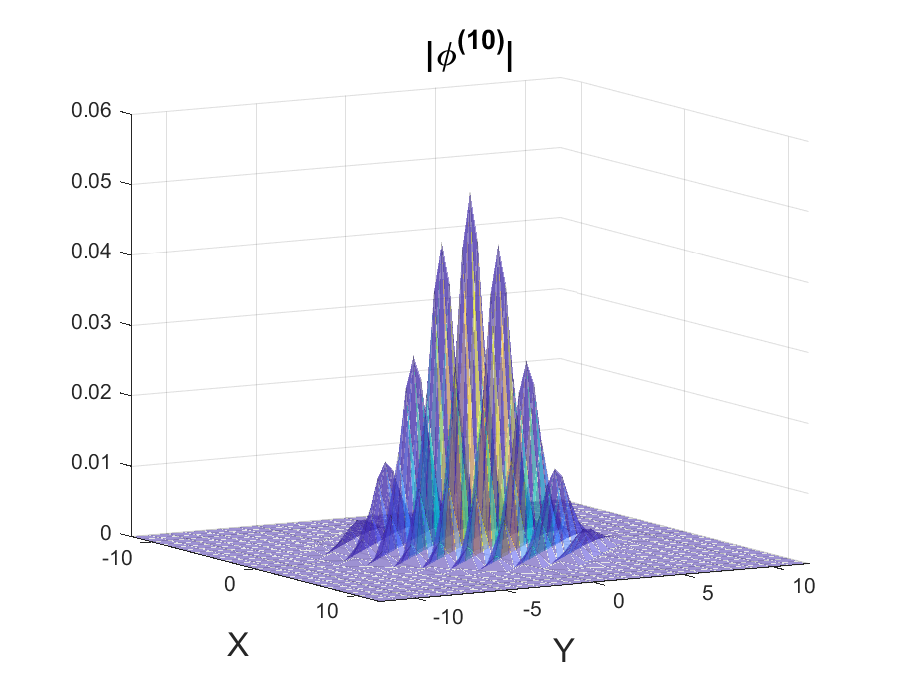
\includegraphics[scale=0.54]{convolve_11.eps}
    \caption{$n = 10$.}
    \end{subfigure}
    \begin{subfigure}{0.49\textwidth}
    \centering
    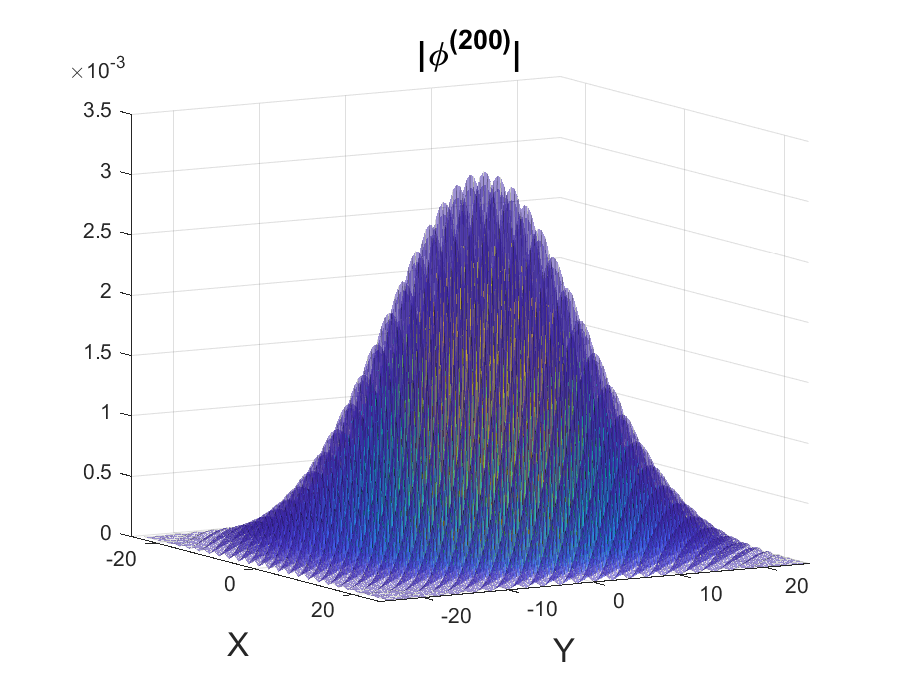
\includegraphics[scale=0.54]{convolve_22.eps}
    \caption{$n = 200$.}
    \end{subfigure}
    \caption{Distribution of $S_n$ for $n=10$ and $n=200$. }
    \label{fig:SRW_convolve}
\end{figure}




\end{example}


\noindent Two interesting concepts in random walk theory are \textbf{recurrence} and \textbf{transience}. A random walk is recurrent
if it visits its starting position infinitely often with probability one and transient if it visits its starting position finitely often with probability one


\begin{framed}
\begin{definition}
Let $\{X_n\}$ be a collection of $\mathbb{Z}^d$-valued i.i.d random vectors with zero mean and consider the associated random walk $\{S_n\}$. We say that the random walk is called \textbf{recurrent} if
\begin{equation*}
    \mathbb{P}(S_n = 0 \text{ for infinitely many } n ) = 1.
\end{equation*}
It is called \textbf{transient} if
\begin{equation*}
    \mathbb{P}(S_n = 0 \text{ for infinitely many } n ) = 0.
\end{equation*}
\end{definition}
\end{framed}
\noindent What's amazing is that the two possibilities of recurrence and transience for a random walk are collectively exhaustive: A random walk is either recurrent or it is transient. This is a consequence of the first and second Borel-Cantelli Lemmas. The following theorem gives a characterization of recurrence and transience in terms of the convolution powers of the distribution $\phi$.

\begin{framed}
\begin{theorem}
The random walk driven by $\phi$ is recurrent if and only if  $\,\sum_{n=1}^\infty \phi^{(n)}(0) = \infty$.
\end{theorem}
\end{framed}



\noindent It can be shown that a simple symmetric random walk on $\mathbb{Z}^d$ is recurrent in dimensions $d = 1, 2$ and transient in dimensions $d \geq 3$. A famous quote by Shizuo Kakutani summarizes this result as follows: ``A drunken man will
always find his way home but a drunken bird may get lost forever.'' Here, we are of course assuming that the motion of both biological entities can be described as simple random walks. For a more thorough description of random walk theory, the reader may refer to \cite{spitzer_principles_1964}.\\



\noindent Fourier analysis allows one to learn about the asymptotic behavior of $\phi^{(n)}$ as $n\to\infty$. For example, when $\phi$ is associated with a random walk that is symmetric, aperiodic, irreducible, or of finite range (The reader may again refer to \cite{spitzer_principles_1964} for more details regarding these terminologies), one may establish the following theorem (Theorem \ref{thm:localglobal}). The first statement concerns the sup-norm behavior of $\phi^{(n)}$ and helps one determine if the random walk is recurrent or transient. The second is the celebrated local limit theorem (originally stated by Abraham de Moivre for independent Bernoulli trials and proved by Pierre-Simon Laplace \cite{mcdonald2005local}). The third is a so-called Gaussian-type estimate.


\begin{framed}
\begin{theorem}\label{thm:localglobal}
Let $\phi$ be a symmetric, aperiodic and irreducible probability distribution on $\mathbb{Z}^d$ with finite variance.
\begin{enumerate}
    \item There are positive constants $C_1, C_2$ for which \begin{equation*}
        \f{C_1}{n^{d/2}} \leq \| \phi^{(n)} \|_\infty \leq \f{C_2}{n^{d/2}}
    \end{equation*}
    for all $n\in \mathbb{N}_+$, where $\| \phi^{(n)} \|_\infty = \sup_{x\in \mathbb{Z}^d} \abs{\phi^{(n)}(x)}$.
    
    \item There exists a simple point-wise description of $\phi^{(n)}$ in the large $n$ limit: The classical local limit theorem states that
    \begin{equation*}
        \phi^{(n)}(x) = \f{1}{n^{d/2}} \Phi_\phi \lp \f{x}{n^{d/2}} \rp + o\lp \f{1}{n^{d/2}} \rp
    \end{equation*}
    uniformly for $x\in \mathbb{Z}^d$, where $\Phi_\phi$ is the generalized Gaussian density
    \begin{equation*}
        \Phi_\phi(x) = \f{1}{(2\pi)^d} \int_{\mathbb{R}^d} \exp\lp -\xi \cdot C_\phi \xi \rp e^{-ix\cdot \xi}\,d\xi = \f{1}{(2\pi)^{d/2} \sqrt{\det C_\phi} }\exp \lp -\f{x\cdot C_\phi^{-1} x }{2} \rp,
    \end{equation*}
    with $C_\phi$ the positive definite covariance matrix associated to $\phi$. 
    
    \item A global point-wise estimate for $\phi^{(n)}$ is the so-called Gaussian estimate: There are positive constants $C$ and $M$ for which
    \begin{equation*}
        \phi^{(n)}(x) \leq \f{C}{n^{d/2}} \exp \lp -\f{M\abs{x}^2}{n} \rp
    \end{equation*}
    for all $x\in \mathbb{Z}^d$ and $n\in \mathbb{N}_+$, where $|\cdot|$ denotes the Euclidean norm. 
\end{enumerate}
\end{theorem}
\end{framed}



\begin{example}\normalfont
To illustrate the claim of the first item of Theorem \ref{thm:localglobal}, we may return to the simple random walk in $\mathbb{Z}^2$ from Example \ref{ex:SRW}. Figure \ref{fig:SRW} shows that $\sup | \phi^{(n)}|$ decays like $1/n$, as expected.

\begin{figure}[!htb]
    \begin{subfigure}{0.49\textwidth}
    \centering
    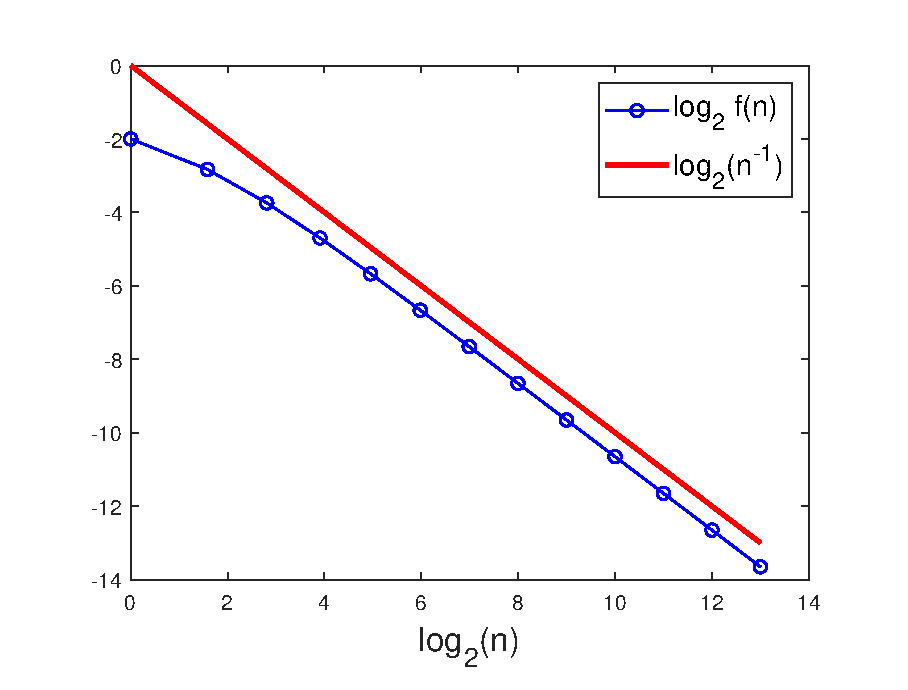
\includegraphics[scale=0.54]{SRW_ex.eps}
    \caption{$n = 300$.}
    \end{subfigure}
    \begin{subfigure}{0.49\textwidth}
    \centering
    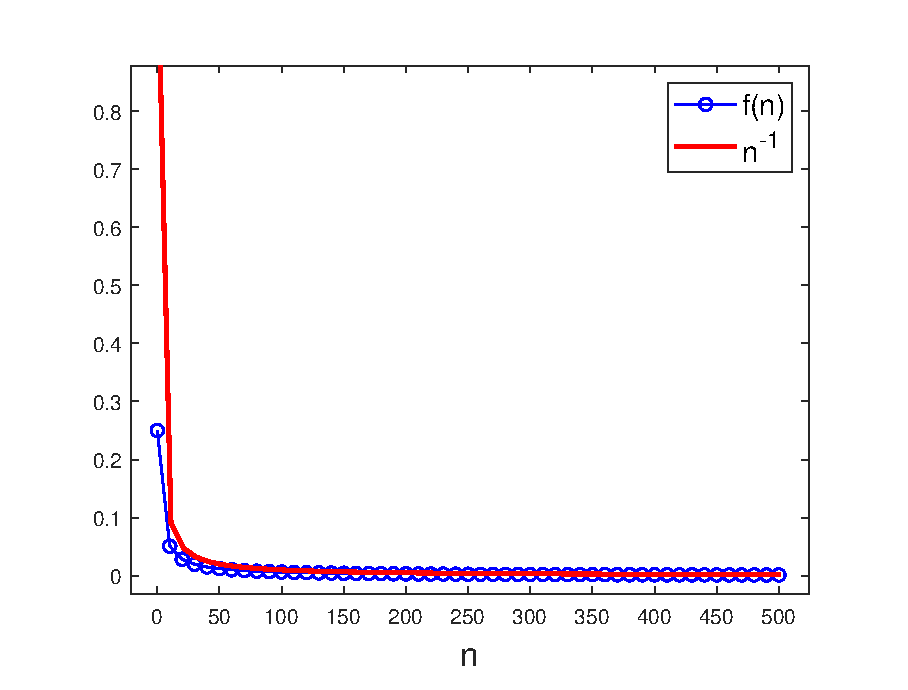
\includegraphics[scale=0.54]{SRW_ex_11.eps}
    \caption{$n = 600$.}
    \end{subfigure}
    \caption{The decay of $f(n)\coloneqq \sup |\phi^{(n)}|$ in $n$. Here, $\phi$ is defined in Example \ref{ex:SRW} for $d=2$.}
    \label{fig:SRW}
\end{figure}
\end{example}





\noindent When $\phi$ is not necessarily a probability distribution, the question of whether one can still obtain global and local/point-wise decay estimates and descriptions of its convolution powers $\phi^{(n)}$ in the large $n$ limit remains valid despite the lack of an underlying stochastic (probabilistic) process \footnote{There is a related generalized notion of ``pseudo-process'' whose steps are driven by ``pseudo random variables" whose distributions are signed (See \cite{lachal2008first}).}.
In the works of Persi Diaconis, Evan Randles, and Laurent Saloff-Coste (see, for example, \cite{randles_convolution_2015}, \cite{randles_convolution_2017}, \cite{diaconis_convolution_2014}), one drops the positivity and real-valuedness of $\phi$, and considers the collection of absolutely summable complex-valued functions $\phi$ defined on the $d$-dimensional integer lattice $\mathbb{Z}^d$, i.e., this is the set of functions $\phi:\mathbb{Z}^d\to\mathbb{C}$ for which
\begin{equation*}
    \| \phi \|_1 = \sum_{x\in \mathbb{Z}^d} \abs{\phi(x)} < \infty.
\end{equation*}
We denote this collection (a Banach space) but $\ell^1(\mathbb{Z}^d)$. For each such $\phi\in\ell^1(\mathbb{Z}^d)$, one can compute its convolution powers\footnote{Equipped with the convolution product, $\ell^1(\mathbb{Z}^d)$ becomes a Banach algebra.} $\phi^{(n)}$ (as done in the probabilistic setting) and study the asymptotic behavior of $\phi^{(n)}$. As illustrated in Example \ref{exp:firstExample}, one still finds rich limiting behaviors of $\phi^{(n)}$, many of which do not appear in the probabilistic setting.


%Example \ref{exp:firstExample} shows the real part of the convolution powers of such a $\phi$ defined on $\mathbb{Z}^2$. 

\begin{example}\label{exp:firstExample}\normalfont
Consider the function $\phi : \mathbb{Z}^2 \to \mathbb{C}$ defined below. Figure \ref{fig:conv_1} shows the real part of $\phi^{(n)}$ for $n=300$ and $n=600$. 
\begin{equation*}
    \phi(x,y) = 
    \f{1}{768}\times
    \begin{cases}
    602 - 112i &(x,y) = (0,0)\\
    56 + 32i   &(x,y) = (-1,0)\\
    72 + 32i   &(x,y) = (1,0)\\
    -16        &(x,y) = (\pm 2,0)\\
    56 + 32i   &(x,y) = (0,\pm 1)\\
    -28 - 8i   &(x,y) = (0,\pm 2)\\
    56         &(x,y) = (0,\pm 3)\\
    -1         &(x,y) = (0,\pm 4)\\
    4          &(x,y) = (-1,\pm 1)\\
    -4         &(x,y) = (1,\pm 1)\\
    0          &\text{otherwise}.
    \end{cases}
\end{equation*}


\begin{figure}[!htb]
    \begin{subfigure}{0.49\textwidth}
    \centering
    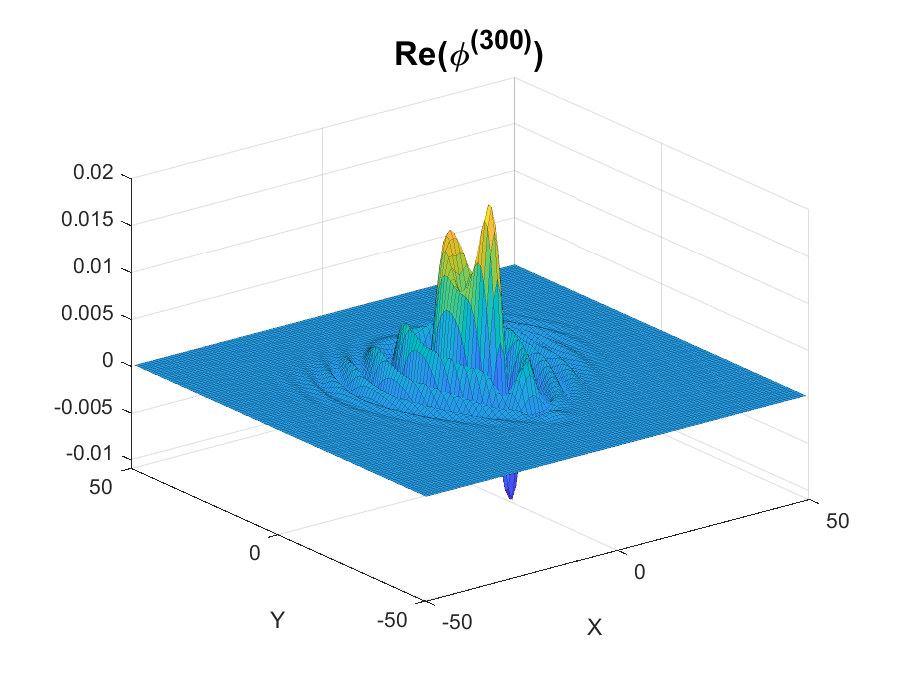
\includegraphics[scale=0.54]{conv_ex0.eps}
    \caption{$n = 300$.}
    \end{subfigure}
    \begin{subfigure}{0.49\textwidth}
    \centering
    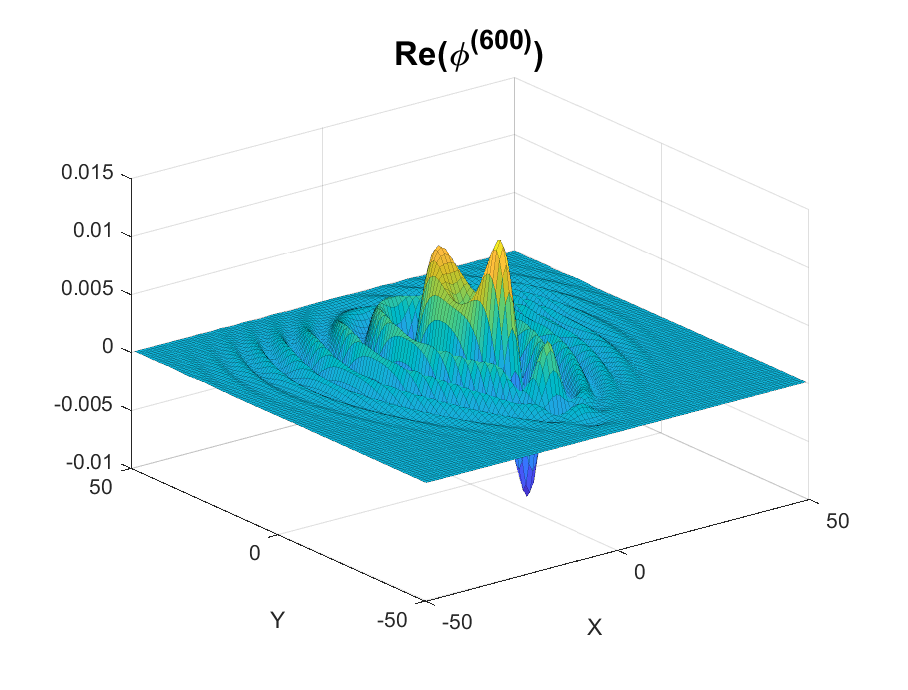
\includegraphics[scale=0.54]{conv_ex1.eps}
    \caption{$n = 600$.}
    \end{subfigure}
    \caption{The real part of $\phi^{(n)}$ for (a) $n=300$ and (b) $n=600$}
    \label{fig:conv_1}
\end{figure}
\end{example}


\noindent In contrast to the probabilistic setting (as see in Example 1 (with your pictures), the non-Gaussian behavior of $\phi^{(n)}$ for a general complex-valued $\phi$ calls for new analysis and theory beyond Theorem 1.2.3.. This is the main objective of the recent papers \cite{randles_convolution_2015}, \cite{randles_convolution_2017}, \cite{diaconis_convolution_2014}, in which great strides have been made towards proving local limit theorems for a large class of sufficiently nice functions $\phi$. In \cite{randles_convolution_2015}, the theory is developed for the case where $\phi$ is defined on $\mathbb{Z}$. Extending earlier works by Thom\'{e}e, de Forest, Schoenberg\footnote{Mathematician Isaac Jacob Schoenberg (1903-1990) was a Romanian-American Assistant Professor of Mathematics at Colby College from 1936 to 1941. He is most well-know for his discovery of mathematical splines --  special functions defined piecewise by polynomials.}, and Greville and using techniques of Fourier analysis, \cite{randles_convolution_2015} not only established asymptotic bounds for the sup-norm of the convolution powers of finitely-supported complex-valued functions on $\mathbb{Z}$ but also proved extended local limit theorems pertaining to this entire class. In \cite{randles_convolution_2017}, a local limit theorem is attained for the case concerning the $d$-dimensional integer lattice; however, it is only applicable to special subset of $\phi$'s. The natural next step is therefore to generalize the result of \cite{randles_convolution_2017} to all admissible $\phi$ on $\mathbb{Z}^d$.\\



\noindent In this thesis, we will mainly be concerned with the question of how the sup-norm of $\phi^{(n)}$ decays in $n$, which is paralleled by Item 1 in Theorem \ref{thm:localglobal}, and our goal is to obtain a global estimate for $\|\phi^{(n)}\|_\infty$. The following theorem (Theorem 1.1 of \cite{randles_convolution_2015}) provides a complete answer for finitely supported functions in $\mathbb{Z}^d$ where $d=1$. 


\begin{framed}
\begin{theorem}[Theorem 1.1 of \cite{randles_convolution_2015}]
Let $\phi : \mathbb{Z} \to \mathbb{C}$ be finitely supported and whose support contains more than one point. Then there is a natural number $m \geq 2$, and positive constants, $A$, $C$, and $C'$ such that 
\begin{equation*}
    Cn^{-1/m} \leq A^{-n}\| \phi^{(n)} \|_\infty \leq C' n^{-1/m}
\end{equation*}
for all natural numbers $n$. Here, $A=\sup|\widehat{\phi}(\xi)|$ where $\widehat{\phi}$ is $\phi$'s Fourier transform, introduced in our Chapter \ref{chap:Estimate-ConvPwr}.
\end{theorem}
\end{framed}

\noindent Theorem 1.4 of \cite{randles_convolution_2017} (Theorem \ref{thm:d} below) treats the $d\geq 1$ case and considers ``sufficiently nice'' rather than an all encompassing class of functions. Its hypotheses will be defined in Chapter \ref{chap:Estimate-ConvPwr}; the objects $\mathcal{S}_d$, $\mu_\phi$, $\Omega(\phi)$ and the notion of positive homogeneous type are due to \cite{randles_convolution_2017} and will be made more precise in the following chapters. The reader may refer to \cite{randles_convolution_2017} for their definitions; however, knowing these definitions is not a prerequisite for what is to come in this paper.

\begin{framed}
\begin{theorem}[Theorem 1.4 of \cite{randles_convolution_2017}]\label{thm:d}
Let $\phi \in \mathcal{S}_d$ be such that $\sup |\widehat{\phi}| = 1$ and suppose that each $\xi \in \Omega(\phi)$ is of positive homogeneous type for $\widehat{\phi}$. Then there are positive constants $\mu_\phi$, $C$, and $C'$ for which 
\begin{equation*}
    C'n^{-\mu_\phi} \leq \| \phi^{(n)} \|_\infty \leq C n^{-\mu_\phi}
\end{equation*}
for all $n\in \mathbb{N}$.
\end{theorem}
\end{framed}

\noindent The main idea of the above result is that, similar to the results of \cite{randles_convolution_2015}, one can obtain a uniform sup-norm bound for the convolution powers of $\phi$ when $d>1$, but under the positive homogeneous condition. One main objective of this thesis is thus to relax this condition and partially extend the above theorem. This requires the generalized polar-coordinate integration formula, which we will formally construct in Chapter \ref{chap:formula}. 







\section{Some notational conventions}
In addition to the conventions outlined in the previous sections, we shall denote by $\mathbb{N}$, and $\mathbb{N}_+$ the set of (non-negative) natural numbers and positive natural numbers, respectively; the $d$-tuples formed by elements of these sets will be denoted by $\mathbb{Z}^d$, $\mathbb{N}^d$, and $\mathbb{N}_+^d$. 
Our setting is $d$-dimensional Euclidean space $\mathbb{R}^d$ with coordinates $(x^1,x^2,\dots,x^d)$ equipped with the dot product and associated Euclidean norm. We take $\mathbb{R}^d$ to be equipped with its usual topology and (oriented) smooth structure. Given $x\in\mathbb{R}^d$ and $R>0$, the open ball with center $x$ and radius $R$ is denoted by $\mathbb{B}_R(x)$ and its corresponding sphere is denoted by $\mathbb{S}_R(x)$. We write $\mathbb{B}=\mathbb{B}_1(0)$ to denote the standard unit ball in $\mathbb{R}^d$. For a subset $A$ of a topological space, we denote by $\Interior{(A)}$, $\overline{A}$, and $\partial A$ its interior, closure and boundary, respectively. We shall denote by $\End(\mathbb{R}^d)$ the collection of linear transformations on $\mathbb{R}^d$ and by $\MdR$ the corresponding set of $d\times d$ real matrices. We denote by $\Gl(\mathbb{R}^d)$ the general linear group and by $\GldR$ the corresponding group of $d\times d$ invertible real matrices. For $E\in \End(\mathbb{R}^d)$ (or $E\in\MdR$), $\|E\|$ will denote the so-called operator norm.










%%%%%%%%%%%%%%%% Pos-Hom Functions %%%%%%%%%%%%%%%%%%%%%%%%%%%%
\chapter{Positive Homogeneous Functions}\label{chap:pos-hom-fns}





\begin{framed}
\begin{proposition}\label{prop:supersub_implies_sub}
Let $Q$ be differentiable on an open neighborhood of $0$ in $\mathbb{R}^d$ and let $E\in\End(\mathbb{R}^d)$ be such that $\{r^E\}$ is a contracting group. If, for some $k\geq 1$, $Q$ is strongly subhomogeneous with respect to $E$ of order $k$ and $Q(0)=0$, then $Q$ is subhomogeneous with respect to $E$.
\end{proposition}
\end{framed}
\begin{proof}
Let $\epsilon>0$ and $K$ be a compact set.  In view of our supposition that $Q$ is strongly subhomogeneous with respect to $E$ or order $k$, let $\delta>0$ be given so that $\abs{r\partial_r Q(r^E\xi)}\leq \epsilon r$ for all $\xi\in K$ and $0<r< \delta$. Given that $r^E$ is a contracting group and $Q(0)=0$, it follows that, for each $\xi\in K$, $f_{\xi}:[0,\delta)\to\mathbb{C}$ defined by
\begin{equation*}
f_{\xi}(r)=\begin{cases}
Q(r^E\xi) & 0<r<\delta\\
0 & r=0
\end{cases}
\end{equation*}
is differentiable on $(0,\delta)$ and continuous on $[0,\delta)$, for each $\xi\in K$. Consequently, for every $0<r<\delta$ and $\xi\in K$, the mean value theorem guarantees a $c=c_{\xi,r}\in (0,r)$ for which 
\begin{equation*}
\abs{f_{\xi}(r)-f_{\xi}(0)}\leq r\abs{f_{\xi}'(c)}=
r\Bigg\vert\partial_r Q(r^E\xi)\Big\vert_{r=c}\Bigg\vert\leq r\epsilon.
\end{equation*}
Consequently, for all $0<r<\delta$ and $\xi\in K$,
\begin{equation*}
\abs{Q(r^E\xi)}=\abs{f_{\xi}(r)-f_{\xi}(0)}\leq r\epsilon.
\end{equation*}
\end{proof}




\begin{framed}
\begin{proposition}\label{prop:Subhomequivtolittleoh}
Let $P$ be positive homogeneous and $\widetilde{P}$ be complex-valued and continuous on a neighborhood of $0$ in $\mathbb{R}^d$. The following are equivalent:
\begin{enumerate}[label=(\alph*), ref=(\alph*)]
    \item\label{item:Subhomequivtolittleoh1} $\widetilde{P}(\xi)=o(P(\xi))$ as $\xi\to 0$.
    \item\label{item:Subhomequivtolittleoh2} For every $E\in\Exp(P)$, $\widetilde{P}$ is subhomogeneous with respect to $E$.
    \item\label{item:Subhomequivtolittleoh3} There exists $E\in\Exp(P)$ for which $\widetilde{P}$ is subhomogeneous with respect to $E$.
\end{enumerate}
\end{proposition}
\end{framed}
\begin{proof}
\begin{subproof}[\ref{item:Subhomequivtolittleoh1} $\Rightarrow$ \ref{item:Subhomequivtolittleoh2}] Let $\epsilon>0$, $K$ be a compact set and choose $E\in \Exp(P)$. Given our supposition that $\widetilde{P}(\xi)=o(P(\xi))$ as $\xi\to 0$, we can find an open neighborhood $\mathcal{O}$ of $0$ for which 
\begin{equation*}
\abs{\widetilde{P}(\xi)}\leq \frac{\epsilon}{1+\sup_{\eta\in K}P(\eta)}P(\xi)
\end{equation*}
for all $\xi\in \mathcal{O}$. Now, because $r^E$ is contracting in view of Proposition \ref{prop:PositiveHomogeneousCharacterization}, we can find a $\delta>0$ for which $r^E\xi\in \mathcal{O}$ for all $0<r<\delta$ and $\xi\in K$ by virtue of Proposition \ref{prop:ContractingCapturesCompact}. Consequently, for all $0<r<\delta$ and $\xi\in K$,
\begin{equation*}
\abs{\widetilde{P}(r^E\xi)}\leq \frac{\epsilon}{1+\sup_{\eta\in K}P(\eta)}P(r^E\xi)=\epsilon r\frac{P(\xi)}{1+\sup_{\eta\in K}P(\eta)}\leq r\epsilon.
\end{equation*}
\end{subproof}

\begin{subproof} [\ref{item:Subhomequivtolittleoh2} $\Rightarrow$ \ref{item:Subhomequivtolittleoh3}] This implication is trivial.
\end{subproof}
 
\begin{subproof}[\ref{item:Subhomequivtolittleoh3} $\Rightarrow$ \ref{item:Subhomequivtolittleoh1}]  Let $\epsilon>0$. Choose $E\in \Exp(P)$ and let $S=\{\eta\in\mathbb{R}^d:P(\eta)=1\}$. Using the supposition that $\widetilde{P}$ is subhomogeneous with respect to $E$, we may choose $\delta>0$ for which
\begin{equation*}
\abs{\widetilde{P}(r^E\eta)}\leq \epsilon r 
\end{equation*}
for all $0<r<\delta$ and $\eta\in S$. We remark that, in view of the continuity of $\widetilde{P}$ and the fact that $r^E$ is contracting, this inequality ensures that $\widetilde{P}(0)=0$. We fix $\mathcal{O}$ to be the open set $B_\delta=\{\xi\in\mathbb{R}^d:P(\xi)<\delta\}$. For each non-zero $\xi\in\mathcal{O}$, we observe that $\xi=r^E\eta$ where $0<r=P(\xi)<\delta$ and $\eta=P(\xi)^{-E}\xi\in S$ and therefore
\begin{equation*}
\abs{\widetilde{P}(\xi)}=\abs{\widetilde{P}(r^E\eta)}\leq r\epsilon=\epsilon  P(\xi)
\end{equation*}
If $\xi=0$, obviously, $\abs{\widetilde{P}(\xi)}=0=\epsilon P(0)=\epsilon P(\xi)$. Thus, for all $\xi\in\mathcal{O}$,
\begin{equation*}
\abs{\widetilde{P}(\xi)}\leq\epsilon P(\xi),
\end{equation*}
as desired.
\end{subproof}
\end{proof}

\begin{framed}
\begin{proposition}\label{prop:2StronglySubhomogeneous}
Let $E\in\End(\mathbb{R}^d)$ be for which $\{r^E\}$ is contracting and suppose that $Q$ is strongly subhomogeneous with respect to $E$ of order $2$. Given $\alpha>0$, set $F=\alpha E$. Then, for any $\epsilon>0$ and compact set $K$,
\begin{equation*}
    \abs{\theta\partial_\theta Q(\theta^F\eta)}\leq \epsilon \theta^\alpha
\end{equation*}
and
\begin{equation*}
    \abs{\theta^2\partial_\theta^2 Q(\theta^F\eta)}\leq \epsilon \theta^\alpha
\end{equation*}
for all $0<\theta\leq \delta^{1/\alpha}$ and $\eta\in K$.
\end{proposition}
\end{framed}
\begin{proof}
Let $\epsilon>0$ and $K\subseteq\mathbb{R}^d$ be a compact set. By virtue of the strong subhomogeneity of $Q$, let $\delta>0$ be such that
\begin{equation*}
    \abs{r\partial_r Q(r^E\eta)}\leq \epsilon' r\hspace{1cm}\mbox{and}\hspace{1cm}\abs{r^2\partial_r^2Q(r^E\eta)}\leq \epsilon' r
\end{equation*}
for $0<r<\delta$ and $\eta\in K$ where $\epsilon'=\epsilon/(2\alpha^2+\alpha)$. We set $r=\theta^\alpha$ so that $r^E=\theta^F$ and observe that
\begin{equation*}
    \abs{\theta\partial_\theta Q(\theta^F\eta)}=\abs{\theta\partial_rQ(r^E\eta)\frac{\partial r}{\partial\theta}}= \abs{\theta\partial_rQ(r^E\eta)\alpha \theta^{\alpha-1}}=\alpha r\abs{\partial_rQ(r^E\eta)}\leq \alpha\epsilon' r<\epsilon \theta^\alpha
\end{equation*}
for all $0<\theta\leq \delta^{1/\alpha}$ and $\eta\in K$. Further, we have
\begin{eqnarray*}
    \abs{\theta^2\partial_\theta^2Q(\theta^F\eta)}&=&\theta^2\abs{\partial_r^2Q(r^E\eta)\left(\frac{\partial r}{\partial\theta}\right)^2+\partial_r Q(r^E\eta)\frac{\partial^2 r}{\partial \theta^2}}\\
    &=&\theta^2\abs{\partial_r^2 Q(r^E\eta) \alpha^2\theta^{2\alpha-2}+\partial_r Q(r^E\eta)\alpha(\alpha-1)\theta^{\alpha-2}}\\
    &\leq &\alpha^2\abs{r^2Q(r^E\eta)}+\abs{\alpha(\alpha-1)}\abs{r\partial_r Q(r^E\eta)}\\
    &< &\alpha^2 \epsilon' r+\abs{\alpha^2-\alpha}\epsilon' r\\
    &<&\epsilon\theta^\alpha
\end{eqnarray*}
for all $0<\theta<\delta^{1/\alpha}$ and $\eta\in K$.
\end{proof}



%%%%%%%%%%%%%%%% Generalized %%%%%%%%%%%%%%%%%%%%%%%%%%%%
\chapter{A generalized polar integration formula}\label{chap:formula}




%%%%%%%%%%%%%%%% Van der Corput  %%%%%%%%%%%%%%%%%%%%%%%%%%%%
\chapter{Van der Corput Lemmas and Estimating Oscillatory Integrals}\label{chap:VanDerCorput}
\chaptermark{VdC Lemmas \& Oscillatory Integrals}
















%%%%%%%%%%%%%%%% Estimating convolution powers  %%%%%%%%%%%%%%%%%%%%%%%%%%%%
\chapter{Application: Estimating convolution powers of complex-valued functions on $\mathbb{Z}^d$}
\label{chap:Estimate-ConvPwr}
\chaptermark{Applications in convolution powers}











\section{Examples}\label{sec:Examples}

%%%%%%%%%%%%%%%%%%%%%%%%%%%%%%%


In this section, we give a number of examples illustrating the results of Theorem \ref{thm:ConvolutionPowerEstimate}, all of which are beyond the scope of validity of the results of \cite{randles_convolution_2017}. First, we treat a useful proposition which gives sufficient conditions for a point $\xi_0\in\Omega(\phi)$ to be of positive homogeneous or imaginary homogeneous type for $\hat{\phi}$ in terms of the Taylor expansion for $\Gamma_{\xi_0}$.


\begin{framed}
\begin{proposition}\label{prop:ExpandGamma}
Let $\phi\in\mathcal{S}_d$ with $\sup_{\xi}|\widehat{\phi}(\xi)|=1$ and let $\xi_0\in\Omega(\phi)$. Suppose that there exists $\mathbf{m}\in \mathbb{N}^d_+$ and some $k \geq 1$ such that the Taylor expansion of $\Gamma_{\xi_0} : \mathcal{U}\to\mathbb{C}$ centered at $0$ is a series of the form
\begin{eqnarray}\label{eq:SemiEllipticImaginaryExpansion}\nonumber
    \Gamma_{\xi_0}(\xi) 
    &=& i\al_{\xi_0} \cdot \xi - i \left( \sum_{\abs{\be : 2\mathbf{m}} \geq 1} A_\be \xi^\be\right) - \sum_{\abs{\be : 2\mathbf{m}} \geq k} B_\be \xi^\be \\ \nonumber
    &=& i\al_{\xi_0} \cdot \xi - i \lp \sum_{\abs{\be : 2\mathbf{m}} = 1} A_\be \xi^\be + \sum_{\abs{\be : 2\mathbf{m}} > 1} A_\be \xi^\be\rp 
    - \lp \sum_{\abs{\be : 2\mathbf{m}} = k} B_\be \xi^\be + \sum_{\abs{\be : 2\mathbf{m}} > k} B_\be \xi^\be \rp \\
    &=&  i\al_{\xi_0} \cdot \xi - i\lp Q_{\xi_0}(\xi) + \widetilde{Q}_{\xi_0}(\xi)\rp - \lp R_{\xi_0}(\xi) + \widetilde{R}_{\xi_0}(\xi) \rp,
\end{eqnarray}
where $\al_{\xi_0} \in \mathbb{R}^d$;   $Q_{\xi_0}$ and $R_{\xi_0}$ are real-valued polynomials for which $R_{\xi_0}$ is positive definite; and  $\widetilde{Q}_{\xi_0},$ and $\widetilde{R}_{\xi_0}$ are real multivariate power series which are absolutely and uniformly convergent on $\mathcal{U}$. If $k=1$, then $\xi_0$ is of positive homogeneous type for $\widehat{\phi}$. If $k>1$ and $|Q_{\xi_0}|$ is positive definite, then $\xi_0$ is of imaginary homogeneous type for $\hat{\phi}$. In either case, $\xi_0$ has drift $\alpha_{\xi_0}$ and homogeneous order
\begin{equation*}
    \mu_{\xi_0}=\abs{\mathbf{1}:2\mathbf{m}}=\sum_{j=1}^d\frac{1}{2m_j}.
\end{equation*}
\end{proposition}
\end{framed}

\noindent Before proving the proposition, we shall first take care of the following useful lemma.

\begin{framed}
\begin{lemma}
Given an open neighborhood $\mathcal{U}$ of $0$ in $\mathbb{R}^d$, suppose that $Q:\mathcal{U}\to\mathbb{C}$ is real-analytic on $\mathcal{U}$ with absolutely and uniformly convergent series expansion
\begin{equation*}
    Q(\xi)=\sum_{|\beta:\mathbf{n}|>1}A_\beta\xi^\beta
\end{equation*}
for some $\mathbf{n}\in\mathbb{N}_+^d$. Consider $E\in\End(\mathbb{R}^d)$ with standard representation $\diag(1/n_1,1/n_2,\dots,1/n_d)$. Then, for each $k\in\mathbb{N}_+$, $Q$ is strongly subhomogeneous with respect to $E$ of order $k$. 
\end{lemma}
\end{framed}
\begin{proof}
It suffices to show that, for each, $j\in\mathbb{N}_+$, $\epsilon>0$ and compact set $K\subseteq\mathbb{R}^d$, there is a $\delta>0$ for which
\begin{equation*}
    \abs{r^j\partial_r^jQ(r^E\eta)}\leq \epsilon r
\end{equation*}
for all $0<r<\delta$ and $\eta\in K$. To this end, we fix $j$, $\epsilon$, and $K$ as above and write $Q=Q_1+Q_2$ where
\begin{equation*}
Q_1(\xi)=\sum_{1+\rho\leq |\beta:\mathbf{n}|\leq 2j+2}A_\beta\xi^\beta
\hspace{0.5cm}\mbox{and}\hspace{0.5cm}
    Q_2(\xi)=\sum_{|\beta:\mathbf{n}|> 2j+2}A_{\beta}\xi^\beta
\end{equation*}
where $\rho:=\min\{|\beta:\mathbf{n}|:A_\beta\neq 0\}-1>0$.
For each $q\geq 1$ and $l\in \mathbb{N}_+$, define
\begin{equation*}
    \mathcal{P}(q,l)=q(q-1)(q-2)\cdots (q-(l-1)).
\end{equation*}
In this notation, we observe that 
\begin{equation*}
    \partial_r^j(r^E\xi)^\beta=\partial_r^j\left(r^{|\beta:\mathbf{n}|}\xi^\beta\right)=\mathcal{P}(|\beta:\mathbf{n}|,j)r^{|\beta:\mathbf{n}|-j}\xi^\beta
\end{equation*}
for $\xi\in\mathbb{R}^d$, $r>0$ and $\beta\in\mathbb{N}^d$.
Because $Q_1$ is a polynomial and $K$ is compact, we have
\begin{equation*}
    M_1:=\sup_{\eta\in K}\lp\sum_{1+\rho\leq |\beta:\mathbf{n}|\leq 2j+2}\abs{A_\beta \mathcal{P}(|\beta:\mathbf{n}|,j)\eta^\beta}\rp<\infty.
\end{equation*}
Given that $Q$ is absolutely and uniformly convergent on $\mathcal{U}$, let $\mathcal{O}\subseteq \overline{\mathcal{O}}\subseteq\mathcal{U}$ be an open neighborhood of $0$ for which
\begin{equation*}
    M_2:=\sup_{\xi\in \mathcal{O}}\lp \sum_{|\beta:\mathbf{n}|>2j+2}\abs{A_\beta\xi^\beta}\rp<\infty.
\end{equation*}
We now specify $\delta$. First, given that $\{r^E\}$ and $\{r^{E/4}\}$ are contracting and the set $K$ is compact, we may find a $0<\delta_1\leq 1$ for which $r^E\eta$ and $r^{E/4}\eta$ belong to $\mathcal{O}$ whenever $0<r<\delta_1$ and $\eta\in K$. Also, there exists $\delta_2>0$ for which
\begin{equation}\label{eq:PermuationEst}
    \abs{\mathcal{P}(q,j)}r^{q/4}\leq 1
\end{equation}
for all $q>j$ and $0<r\leq \delta_2$; it is sufficient to take $\delta_2=e^{-4j}$.  Finally, given that $\rho>0$, let $\delta_3>0$ be such that
\begin{equation*}
    M_1 r^\rho+M_2r<\epsilon
\end{equation*}
for all $0<r<\delta_3$. Set $\delta=\min\{\delta_1,\delta_2,\delta_3\}$ and observe that
for all $\eta\in K$ and $0<r<\delta$, we have
\begin{eqnarray*}
    \abs{r^j\partial_r^jQ_1(r^E\eta)}&=&r^j\abs{\sum_{1+\rho\leq|\beta:\mathbf{n}|\leq 2j+2}A_\beta \partial_r^j\lp r^E\eta\rp^{\beta}}\\
    &\leq&r^j\sum_{1+\rho\leq|\beta:\mathbf{n}|\leq 2j+2}\abs{A_\beta\mathcal{P}(|\beta:\mathbf{n}|,j)r^{|\beta:\mathbf{n}|-j}\eta^\beta}\\
    &\leq&r^{1+\rho}\sum_{1+\rho\leq |\beta:\mathbf{n}|\leq 2j+2}\abs{A_\beta \mathcal{P}(|\beta:\mathbf{n}|,j)\eta^\beta}\\
&\leq&r  M_1r^\rho.
\end{eqnarray*}
By virtue of \eqref{eq:PermuationEst}, for each $q=|\beta:\mathbf{n}|>2j+2$, we have
\begin{eqnarray*}
    \abs{\partial_r^j\lp A_\beta(r^E\eta)^\beta\rp}&=&\abs{A_\beta}\abs{\mathcal{P}(|\beta:\mathbf{n}|,j)}r^{|\beta:\mathbf{n}|-j}\abs{\eta^\beta}\\
    &=&r^{|\beta:\mathbf{n}|/2-j}\abs{A_\beta}\abs{\mathcal{P}(|\beta:\mathbf{n}|,j)r^{|\beta:\mathbf{n}|/4}}\abs{(r^{E/4}\eta)^\beta}\\
    &\leq& r\abs{A_\beta(r^{E/4}\eta)^\beta}
\end{eqnarray*}
for all $0<r<\delta\leq\delta_2$ and $\eta\in K$. It follows that
\begin{eqnarray*}
    \abs{\partial_r^jQ_2(r^E\eta)}&=&\abs{\sum_{|\beta:\mathbf{n}|> 2j+2}\partial_r^j\lp A_\beta(r^E\eta)^\beta\rp}\\
    &\leq & \sum_{|\beta:\mathbf{n}|>2j+2}\abs{\partial_r^j\lp A_\beta(r^E\eta)^\beta\rp}\\
    &\leq&\sum_{|\beta:\mathbf{n}|>2j+2}r\abs{A_\beta(r^{E/4}\eta)^\beta}\\
    &\leq &rM_2
\end{eqnarray*}
for all $0<r<\delta$ and $\eta\in K$. Therefore, for each $0<r<\delta$ and $\eta\in K$, we have
\begin{eqnarray*}
    \abs{r^j\partial_r^jQ(r^E\eta)}&\leq&\abs{r^j\partial_r^jQ_1(r^E\eta)}+\abs{r^j\partial_r^jQ_2(r^E\eta)}\\
    &\leq& rr^\rho M_1+r^{j+1}M_2\\
    &\leq& r(M_1r^\rho+M_2r)\\
    &<&r \epsilon.
\end{eqnarray*}
\end{proof}

\begin{proof}[Proof of Proposition \ref{prop:ExpandGamma}.]
It is easy to see that $E\in \Exp(Q_{\xi_0})\cap\Exp(\abs{Q_{\xi_0}})$ and $E/k\in\Exp(R_{\xi_0})$ for $E\in\End(\mathbb{R}^d)$ with standard matrix representation 
\begin{equation*}
\diag((2m_1)^{-1}, (2m_2)^{-1},\dots, (2m_d)^{-1}).
\end{equation*}
If $k=1$, $R_{\xi_0}$ is positive homogeneous with $E\in\Exp(R_{\xi_0})\cap\Exp(Q_{\xi_0})$. By virtue of the preceding lemma (with $\mathbf{n}=2\mathbf{m}$), $\widetilde{Q}_{\xi_0}$ and $\widetilde{R}_{\xi_0}$ are strongly subhomogeneous with respect to $E$ of order $1$ and so, in view of Proposition \ref{prop:supersub_implies_sub}, both are subhomogeneous with respect to $E$. In this case, we may conclude that $\xi_0$ is of positive homogeneous type for $\widehat{\phi}$ with drift $\alpha_{\xi_0}$ and homogeneous order
\begin{equation*}
    \mu_{\xi_0}=\tr E=|\mathbf{1}:2\mathbf{m}|=\sum_{j=1}^d\frac{1}{2m_j}.
\end{equation*}
If $k>1$, our supposition guarantees that $\abs{Q_{\xi_0}}$ is positive homogeneous with respect to $E$ and $R_{\xi_0}$ is positive homogeneous with respect to $E/k$. By virtue of the preceding lemma, $\widetilde{Q}_{\xi_0}$ is strongly subhomogeneous with respect to $E$ of order $2$ and $\widetilde{R}_{\xi_0}$ is strongly subhomogeneous with respect to $E/k$ of order $1$. Consequently, $\xi_0$ is of imaginary homogeneous type for $\widehat{\phi}$ with drift $\alpha_{\xi_0}$ and homogeneous order $\mu_{\xi_0}=\tr E$ as in the previous case.
\end{proof}
%%%%%%%%%%%%%%%%%%%%%%%%%%%%%%%%%%%%%%





\begin{example}\normalfont


Consider the function $\phi : \mathbb{Z}^2 \to \mathbb{C}$ defined by 
\begin{equation*}
    \phi(x,y) =
    \frac{1}{512}\times
    \begin{cases}
    372 - 96i &(x,y) = (0,0)\\
    56+32i &(x,y) = (\pm 1, 0)\mbox{ or }(0,\pm 1)\\
    -28-8i        &(x,y) = (\pm 2,0)\mbox{ or }(0,\pm 2)\\
    8       &(x,y) = (\pm 3,0)\mbox{ or }(0,\pm 3)\\
    -1        &(x,y) = (\pm 4,0)\mbox{ or }(0,\pm 4)\\
    0& \text{otherwise}.
    \end{cases}
\end{equation*}
It is easily verified that $\sup_{\xi}|\widehat{\phi}|=1$ and $\Omega(\phi) = \{\xi_0 \}$ where $\xi_0=(0,0)$. Since $\phi$ is finitely supported, $\Gamma_{0}=\Gamma_{\xi_0}$ is $\mathbb{C}^2$ analytic on its domain and so its Taylor series converges absolutely and uniformly on an open neighborhood $\mathcal{U}\subseteq \mathbb{R}^2$ of $0$. By a straightforward computation, we find 
\begin{eqnarray*}
\Gamma_{0}(\xi)
&=& 
-i\lp \frac{\tau^4}{64} + \frac{\zeta^4}{64}   \rp
-i \sum_{|\beta:(4,4)|\geq 2}A_\beta \xi^\beta\\
&& 
\hspace{1.3cm}
-\lp \f{15\tau^8}{8192} - \f{\tau^4\zeta^4}{4096} + \f{15\zeta^8}{8192}   \rp 
- \sum_{|\beta:(4,4)|\geq 6}B_\beta \xi^\beta\\
&=&-i\lp Q_{0}(\xi)+\widetilde{Q}_{0}(\xi)\rp-\lp R_0(\xi)+\widetilde{R}_0(\xi)\rp
\end{eqnarray*}
where
\begin{equation*}
Q_{0}(\xi)=\sum_{|\beta:(4,4)|=1}A_\beta \xi^\beta=\frac{\tau^4}{64} + \frac{\zeta^4}{64} ,
\end{equation*}
\begin{equation*}
R_{0}(\xi)=\sum_{|\beta:(4,4)|=2}B_\beta\xi^\beta
=  \f{15\tau^8}{8192} - \f{\tau^4\zeta^4}{4096} + \f{15\zeta^8}{8192}  , 
\end{equation*}
\begin{equation*}
\widetilde{Q}_{0}(\xi)= \sum_{|\beta:(4,4)| \geq 3/2}A_\beta \xi^\beta= 
-\f{\tau^6+\zeta^6}{384}  + \f{\tau^8 + \zeta^8}{5120}+  \f{7(\tau^4\zeta^8+\tau^8\zeta^4)}{262144} +
\cdots, 
\end{equation*}
and
\begin{eqnarray*}
\widetilde{R}_{0}(\xi)=\sum_{|\beta:(4,4)|\geq 5/2}B_\beta \xi^\beta 
=\f{(\tau^4\zeta^6 + \tau^6\zeta^4)}{24576} - \f{\tau^6\zeta^6}{147456} - \f{(\tau^4\zeta^8 + \tau^8\zeta^4)}{327680}
\cdots, 
\end{eqnarray*}
for $\xi=(\tau,\zeta)\in\mathcal{U}$. Observe that this expansion is of the form \eqref{eq:SemiEllipticImaginaryExpansion} with $\alpha_0=(0,0)$, $\mathbf{m}=(2,2)$, and $k=2$. It is readily verified that $|Q_0|=Q_0$ and $R_0$ are positive definite and, by virtue of Proposition \ref{prop:ExpandGamma}, we conclude that $\xi_0=0$ is of imaginary homogeneous type for $\widehat\phi$ with drift $\alpha_0=0$ and homogeneous order
\begin{equation*}
    \mu_{\phi}=\mu_0=|\mathbf{1}:2\mathbf{m}|=\frac{1}{4}+\frac{1}{4}=\f{1}{2}.
\end{equation*}
By an appeal to Theorem \ref{thm:ConvolutionPowerEstimate} we obtain, to each compact set $K\subseteq\mathbb{R}^2$, a positive constant $C$ for which
\begin{equation}\label{eq:SecondOrderExampleDecay}
    |\phi^{(n)}(x,y)|\leq \frac{C}{n^{\mu_\phi}}=\frac{C}{n^{1/2}}
\end{equation}
for all $n\in\mathbb{N}_+$ and $(x,y)\in K$. To illustrate this result, we consider the compact set $K = [-700, 700] \times [-700, 700]$ and define $f(n)=f_{\phi,K}(n)=\max_{(x,y)\in K}\abs{\phi^{(n)}(x,y)}$. Figure \ref{fig:Conv_Pwr_0_new} illustrates this result by capturing the decay of $f(n)=f_{\phi,K}(n)=\max_{(x,y)\in K}\abs{\phi^{(n)}(x,y)}$ relative to that of $n^{-\mu_\phi}$. Also, Figure \ref{fig:Conv_Pwr_00_new} illustrates the graph of $\Re \phi^{(n)}(x,y)$ for $(x,y)\in K$ and $n=200$ and $n=1000$.


\begin{figure}[!htb]
    \begin{subfigure}{0.49\textwidth}
    \centering
    
\includegraphics[scale=0.58]{Fig5a.eps}
    \caption{$\log_2 f(n)$ and $\log_2 n^{-1/2}$ versus $\log_2 n$}
    \end{subfigure}
    \begin{subfigure}{0.49\textwidth}
    \centering
    
\includegraphics[scale=0.58]{Fig5b.eps}
    \caption{$f(n)$ and $n^{-1/2}$ versus $n$}
    \end{subfigure}
    \caption{Behavior of $f(n)=f_{\phi,K}(n)=\max_{(x,y)\in K}\abs{\phi^{(n)}(x,y)}$}
    \label{fig:Conv_Pwr_0_new}
\end{figure}


\begin{figure}[!htb]
    \begin{subfigure}{0.49\textwidth}
    \centering
    
\includegraphics[scale=0.58]{Fig6a.eps}
    \caption{$n = 100$.}
    \label{fig:Conv_Pwr_00a}
    \end{subfigure}
    \begin{subfigure}{0.49\textwidth}
    \centering
    
\includegraphics[scale=0.58]{Fig6b.eps}
    \caption{$n = 1000$.}
    \label{fig:Conv_Pwr_00b}
    \end{subfigure}
    \caption{$\Re\phi^{(n)}(x,y)$ for $n=200$ and $1000$}
    \label{fig:Conv_Pwr_00_new}
\end{figure}
\end{example}










%%%%%%%%%%%%%%%%%%%%%%%%%%



%%%%%%%%%%%%%%%% Appendix  %%%%%%%%%%%%%%%%%%%%%%%%%%%%
\chapter{Appendix}\label{chap:Appendix}





%%%%%%%%%%%%%%%%%%%%%%%%%%%%%%%%%%%%%%%%%%%%%%%%%%
%%%%%%%%%%%%%%%%%%%%%%%%%%%%%%%%%%%%%%%%%%%%%%%%%%%
%%%%%%%%%%%%%%%% Bibliography %%%%%%%%%%%%%%%%%%%%

\bibliographystyle{abbrv}
\bibliography{GPIF}





\end{document}